% ----------------- CHAPTER 4 -----------------

\chapter{Experimental Evaluation}

\section{Experimental Setup}

\subsection{Dataset and Preprocessing}
\indent

All experiments are conducted on the CIFAR-10 dataset~\cite{krizhevsky2009learning}, which contains 50,000 training images and 10,000 testing images across 10 classes.
Images are first normalized to the range $[0,1]$. When applying adversarial perturbations, the perturbation budget $\epsilon$ is calculated relative to this scale, e.g., $2\text{px} = 2.0/255$ and $8\text{px} = 8.0/255$.
After perturbation, inputs are further normalized by subtracting the per-channel mean (0.485, 0.456, 0.406) and dividing by the per-channel standard deviation $0.225$. This normalization procedure aligns with the preprocessing used in \cite{wong2018scaling} for their LP-certified pre-trained models. It ensures consistent input distribution between standard and certified models.

\subsection{Standard Model Training}
\indent

We utilize three architectures previously described in Section~\ref{sec:methodology-models}: Small, Large, and ResNet.  
To provide a fair comparison with the LP-certified models, we train six standard (non-certified) models: two per architecture, using different checkpoints to increase ensemble diversity, as suggested in~\cite{fort2024ensemble}. The training procedure follows a standard supervised classification pipeline using cross-entropy loss and the Adam optimizer.  
Specifically, we train for 20 epochs with a learning rate of 0.001 and a batch size of 128, saving model checkpoints every 10 epochs to capture intermediate models.


\noindent


\begin{algorithm}[H]
\caption{Training and Evaluation Framework}
\label{alg:train_eval}
\begin{algorithmic}
\State \textbf{Require:} \\ Training data $\mathcal{D}_{\text{train}}$, test data $\mathcal{D}_{\text{test}}$, model $f_\theta$, learning rate $\eta$, number of epochs $T$, checkpoint interval $K$

\State \textbf{Training:} \\ Initialize model parameters $\theta$
\For{epoch $=1$ to $T$}
    \State Update $\theta$ by minimizing cross-entropy loss on $\mathcal{D}_{\text{train}}$ using Adam with step size $\eta$
    \State Evaluate current model on $\mathcal{D}_{\text{train}}$ and $\mathcal{D}_{\text{test}}$
    \If{$epoch \bmod K = 0$}
        \State Save model checkpoint with epoch identifier
    \EndIf
\EndFor
\Statex
\Function{Evaluate}{$f_\theta, \mathcal{D}$}
    \State Compute accuracy of $f_\theta$ on dataset $\mathcal{D}$ without parameter updates
\EndFunction
\end{algorithmic}
\end{algorithm}


The overall training and evaluation process is summarized in Algorithm~\ref{alg:train_eval}. During training, model parameters are updated epoch by epoch, and after each epoch we record both training and test accuracy to monitor convergence.  
To enable ensemble construction, we additionally save intermediate model checkpoints every $K=10$ epochs.  
This design allows us to extract diverse models from different stages of the training trajectory, following the approach suggested by~\cite{fort2024ensemble}.  
For our experiments, we retain checkpoints at epoch 10 and epoch 20, which form the two members of each standard ensemble.  
The test accuracies of these checkpoints are reported in Table~\ref{tab:standard_acc}.

\begin{table}[H]
\centering
\caption{Test Accuracy of Standard Models at Different Epochs}
\label{tab:standard_acc}
\begin{tabular}{lcc}
\toprule
Model & Epoch 10 & Epoch 20 \\
\midrule
ResNet & 77.81\% & 81.38\% \\
Large  & 78.04\% & 81.90\% \\
Small  & 65.49\% & 65.49\% \\
\bottomrule
\end{tabular}
\end{table}

This diversity in checkpoints aims to provide complementary networks within the ensemble models, similar in spirit to the LP-certified model set.

\subsection{Threat Model: AutoAttack}
\label{sec:threat model}
\indent

We adopt \texttt{AutoAttack}~\cite{croce2020reliable} to evaluate model robustness under an $\ell_\infty$-bounded white-box threat model. Given a clean input $x \in [0,1]^n$ and classifier prediction $C(x)$, the adversary aims to construct an adversarial input $x' = x + \delta$ that causes misclassification, while ensuring that the perturbation $\delta$ remains imperceptible.

Unlike hand-tuned attacks with sensitive hyperparameters, AutoAttack is a parameter-free ensemble adversary composed of four strong components: \texttt{APGD-CE}, \texttt{APGD-DLR}, \texttt{FAB}, and \texttt{Square Attack}. These cover both gradient-based and gradient-free strategies, improving reliability in robustness evaluation.

\paragraph{Attack Budget}

We adopt standard $\ell_\infty$ budgets with $\epsilon \in \{2/255, 4/255,6/255, 8/255\}$, which bound the allowed perturbation per pixel. AutoAttack strictly enforces this norm constraint during adversarial generation. Thus, any successful attack implies that the resulting adversarial example lies within the $\epsilon$-ball around the clean input.

\paragraph{Parameterization}

In our experiments, AutoAttack is configured with the following specific parameters to ensure a robust and reproducible evaluation:

\begin{itemize}
    \item \textbf{APGD (Auto-PGD)}: Runs with 5 random restarts and 100 iterations each. It uses an untargeted attack setting with no verbosity, a single expectation over transformation iteration, step size scaling factor \(\rho = 0.75\), and the same random seed for reproducibility. The perturbation budget \(\epsilon\) and norm type (\(\ell_\infty\) or \(\ell_2\)) are aligned with the experimental setup.
    
    \item \textbf{FABAttack\_PT}: Configured with 5 restarts, 100 iterations, the specified perturbation budget \(\epsilon\), and norm type. The attack runs silently with a fixed random seed.
    
    \item \textbf{SquareAttack}: Uses a starting perturbation probability \(p_{\text{init}}=0.8\), a maximum of 5000 queries per restart, a single restart, and the same perturbation budget and norm. The schedule for resizing is disabled.
    
    \item \textbf{Targeted APGD}: Runs with a single restart, 100 iterations, and shares the same other parameters as APGD.
\end{itemize}

All attacks use the same device and logging configuration and operate deterministically under a fixed random seed to guarantee reproducibility and fairness. Verbosity is turned off for cleaner experimental logs.


\paragraph{Adversary Capabilities}

We assume a white-box setting where the adversary has full access to the model architecture, weights, and gradients. Attacks are launched on clean test inputs, and perturbations are constrained to lie in the valid input range $[0,1]^n$. The adversary does not leverage knowledge of any certified bounds, defense mechanisms, or training data distribution.

\subsection{Surrogate Model}
\label{sec:surrogate model}
\indent

As mentioned in \cite{zhang2024evaluating} that gradient masking might lead to unrealistic robustness, we need to avoid gradient masking caused by CrossMax. In order to apply AutoAttack to non-differentiable ensemble-based defenses such as Majority Voting and CrossMax, we follow the common practice of attacking a surrogate model similar in \cite{zhang2024evaluating}. We construct a differentiable surrogate model that approximates the ensemble’s behavior.

Specifically, given an ensemble of $M$ base classifiers $\{f_i\}_{i=1}^M$, we define a surrogate model $f_{\text{avg}}$ that averages their logit outputs. Formally, for a given input $x$, the surrogate model outputs:

\begin{equation}
f_{\text{avg}}(x) = \frac{1}{M} \sum_{i=1}^M f_i(x),
\end{equation}

\noindent where each $f_i(x) \in \mathbb{R}^C$ denotes the logit vector produced by the $i$-th model.

This averaged logit surrogate preserves differentiability and provides a tractable target for AutoAttack. Once adversarial examples are generated against $f_{\text{avg}}$, they are evaluated against the true ensemble method (e.g., CrossMax or voting schemes). This approach ensures that adversarial perturbations remain realistic and transferable while maintaining full white-box access to the underlying base models.

\section{Experimental Results and Analysis}

\subsection{Performance of Individual Models}
\indent

Tables~\ref{tab:lp_robust_accuracy_detailed} and \ref{tab:std_robust_accuracy_detailed} present the robust accuracy (\%) of individual models trained with LP-certified and standard training methods on the CIFAR-10 dataset. The evaluation is performed under different adversarial perturbation budgets(threat model details in Section~\ref{sec:threat model}), measured in terms of the maximum allowed $\ell_\infty$ perturbation, denoted as $\epsilon$.

From the tables, we can find out that:

\begin{itemize}
  \item The LP-trained models consistently achieve substantially higher empirical robust accuracy than their standard-trained counterparts across all perturbation budgets, excluding clean inputs.
  \item For LP-trained models, the clean accuracy ranges from approximately 27\% (small 8px model) to 68\% (large 2px model), while robust accuracy gradually decreases as the perturbation budget increases.
  \item In contrast, standard-trained models exhibit a sharp decline in robust accuracy even at low perturbation budgets, falling below 5\% accuracy beyond $\epsilon = 4.0/255$.
  \item The results highlight the effectiveness of LP-certified training in enhancing adversarial robustness, especially at moderate perturbation strengths.
\end{itemize}

\begin{table}[h]
\small
\centering
\caption{Robust Accuracy (\%) of LP-trained Models on CIFAR-10 under Different $\epsilon$.}
\label{tab:lp_robust_accuracy_detailed}
\begin{tabular}{lcccccc}
\toprule
\textbf{Epsilon} & \textbf{Small 2px} & \textbf{Small 8px} & \textbf{Large 2px} & \textbf{Large 8px} & \textbf{ResNet 2px} & \textbf{ResNet 8px} \\
\midrule
Clean (0px) & 60.86 & 27.60 & 67.71 & 19.01 & 66.33 & 27.05 \\
2px & 50.23 & 25.62 & 58.77 & 18.48 & 57.25 & 25.81 \\
4px & 40.30 & 24.12 & 48.47 & 17.80 & 48.00 & 24.73 \\
6px & 30.80 & 22.73 & 38.39 & 17.15 & 38.94 & 23.60 \\
8px & 22.48 & 21.34 & 28.76 & 16.48 & 30.28 & 22.48 \\
\bottomrule
\end{tabular}
\end{table}

\vspace{1em}

\begin{table}[h]
\small
\centering
\caption{Robust Accuracy (\%) of Standard-trained Models on CIFAR-10 under Different $\epsilon$.}
\label{tab:std_robust_accuracy_detailed}
\begin{tabular}{lcccccc}
\toprule
\textbf{Epsilon} & \textbf{Small 1} & \textbf{Small 2} & \textbf{Large 1} & \textbf{Large 2} & \textbf{ResNet 1} & \textbf{ResNet 2} \\
\midrule
Clean (0px) & 65.50 & 69.50 & 81.90 & 78.04 & 81.38 & 77.81 \\
2px & 18.66 & 15.64 & 23.25 & 15.14 & 3.28 & 0.98 \\
4px & 2.23 & 1.00 & 2.17 & 0.39 & 0.00 & 0.00 \\
6px & 0.16 & 0.04 & 0.13 & 0.00 & 0.00 & 0.00 \\
8px & 0.02 & 0.01 & 0.00 & 0.00 & 0.00 & 0.00 \\
\bottomrule

\end{tabular}
\end{table}

\vspace{1em}

\textbf{Notes:} In these tables, the perturbation budget $\epsilon$ (denoted as ``px'') indicates the maximum allowed perturbation under the $\ell_\infty$ norm, scaled to $[0,1]$. For instance, $8\text{px}$ corresponds to $\epsilon = 8.0/255$. The robust accuracy values reflect the empirical accuracy of the model under adversarial attacks bounded by these budgets.


\begin{figure}[htbp]
    \centering
    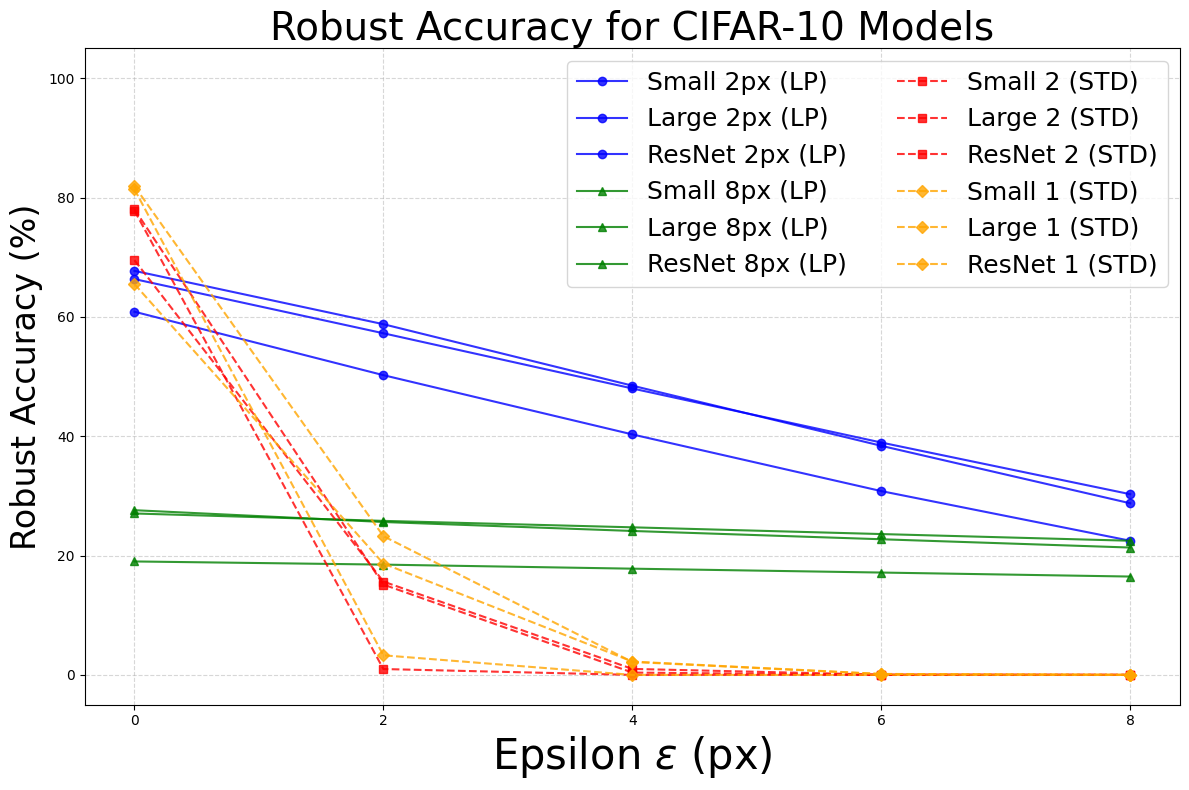
\includegraphics[width=0.85\linewidth]{images/Single model performance.png}
    \caption{Robust accuracy (\%) of LP- and standard-trained CIFAR-10 models under varying perturbation budgets $\epsilon$. LP-trained models (2px and 8px) are shown in blue/green solid lines with circle/triangle markers; standard-trained models (different checkpoints) are shown in red/orange dashed lines with square/diamond markers.}
\label{fig:robust_accuracy}

\end{figure}

\paragraph{Influence of LP Training on Robust Accuracy}  
Figure~\ref{fig:robust_accuracy} illustrates the robust accuracy trends of twelve individual models evaluated on the CIFAR-10 test set under progressively increasing adversarial perturbation budgets $\epsilon$, ranging from clean accuracy ($0px$) to a maximum perturbation setting.

Key observations include:  
\begin{itemize}
    \item \textbf{Trade-off between clean accuracy and robustness:} LP-trained models exhibit lower clean accuracy (accuracy at $\epsilon=0$) compared to standard-trained models. This reflects the known trade-off where improving certified robustness through LP training often entails some loss in clean accuracy~\cite{wong2018provable}.
    \item \textbf{Effect of training perturbation budget within LP models:} Among LP models, those trained with a smaller perturbation budget ($2\text{px}$) generally achieve higher accuracy under low perturbations but degrade more rapidly as $\epsilon$ increases, showing a near-linear decline. Conversely, LP models trained with a larger budget ($8\text{px}$) maintain more stable accuracy across perturbation levels, exhibiting less sensitivity to stronger attacks despite starting with lower clean accuracy.
    \item \textbf{Comparative robustness:} Standard-trained models demonstrate significantly poorer robustness, with sharp drops in accuracy even at the smallest evaluated perturbation budget ($2\text{px}$), and nearly zero accuracy at larger budgets. This stark contrast emphasizes the effectiveness of LP training in defending against adversarial perturbations.
\end{itemize}

These trends highlight two fundamental trade-offs in adversarial robustness research:  
(1) \textit{Robustness vs. clean accuracy trade-off}, where certified robust training methods sacrifice some clean accuracy for robustness gains;  
(2) \textit{Perturbation budget trade-off}, where training with larger budgets increases robustness but at the cost of clean accuracy and overall accuracy under small perturbations.



\begin{figure}[htbp]
    \centering
    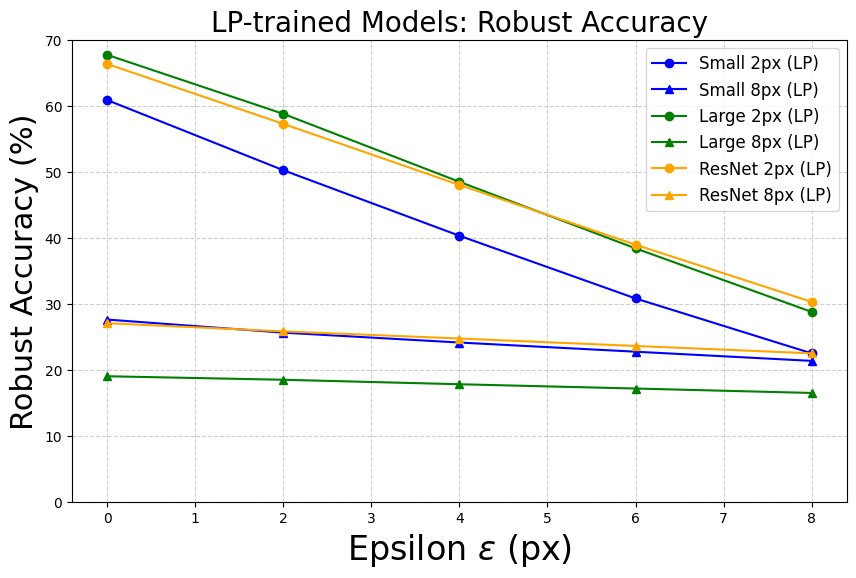
\includegraphics[width=0.80\linewidth]{images/LP_MODEL_STRUCTURE.png}
    \caption{Robust accuracy (\%) of LP-trained models on CIFAR-10 under varying perturbation budgets $\epsilon$ for different architectures: Small, Large, and ResNet. Each line corresponds to a model trained with either 2px or 8px perturbation budget.}
    \label{fig:lp_model_structure}
\end{figure}

\begin{figure}[htbp]
    \centering
    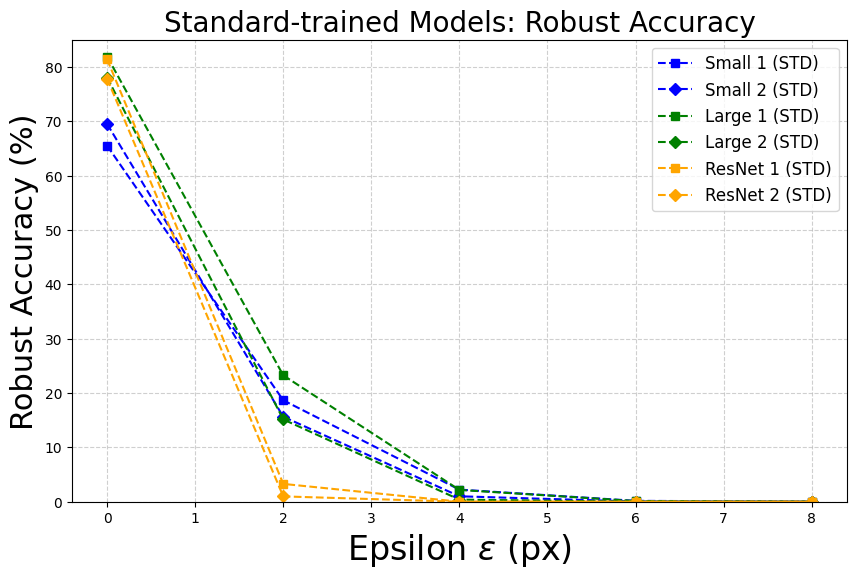
\includegraphics[width=0.80\linewidth]{images/STD_MODEL_STRUCTURE.png}
    \caption{Robust accuracy (\%) of standard-trained models on CIFAR-10 under varying perturbation budgets $\epsilon$ for different architectures: Small, Large, and ResNet.}
    \label{fig:std_model_structure}
\end{figure}

\paragraph{Model Structure Impact on Robust Accuracy}

Figures~\ref{fig:lp_model_structure} and~\ref{fig:std_model_structure} illustrate the robust accuracy of different model architectures (Small, Large, ResNet) under varying perturbation budgets $\epsilon$ for LP-trained and standard-trained models respectively.

For the \textbf{LP-trained models} (Figure~\ref{fig:lp_model_structure}), we observe the following trends:

\begin{itemize}
    \item Under the \textbf{2px training budget}, the \textit{Small} model consistently achieves approximately 8\% lower robust accuracy compared to the \textit{Large} and \textit{ResNet} architectures. This suggests that for smaller perturbation budgets, the \textit{Small} model’s capacity might limit its robustness.
    \item When trained under the \textbf{8px perturbation budget}, the \textit{Large} model exhibits roughly 8\% lower robust accuracy than both the \textit{Small} and \textit{ResNet} models. This may indicate that the \textit{Large} model struggles to maintain accuracy when trained on larger perturbations, potentially due to over-regularization or optimization difficulties at higher budgets.
    \item Across both training budgets, the \textit{ResNet} model shows relatively stable and competitive robustness, closely matching or slightly outperforming the \textit{Small} model under the 8px budget.
\end{itemize}

These observations highlight a nuanced trade-off where model size and architecture influence robustness differently depending on the adversarial training perturbation scale.

For the \textbf{standard-trained models} (Figure~\ref{fig:std_model_structure}), the trends differ significantly:

\begin{itemize}
    \item The \textit{ResNet} models suffer the steepest decline in robust accuracy as perturbation size increases, indicating lower inherent robustness under adversarial attacks without specialized training.
    \item The \textit{Large} model follows with the second fastest decline, while the \textit{Small} model maintains the slowest rate of degradation, albeit at generally low robust accuracy levels.
\end{itemize}

In summary, the impact of model structure on robustness is highly context-dependent. LP training significantly boosts robustness overall, but the choice of architecture and training perturbation budget jointly determine the precise robustness profile. Conversely, without robust training, smaller models show relatively better stability against increasing perturbations despite lower absolute accuracy.






\subsection{Ensemble Methods vs. Best Single Model}
\indent

To evaluate the performance and characteristics of different ensemble methods under adversarial perturbations, we adopt the threat model described in Section~\ref{sec:threat model} and consider multiple perturbation budgets. 
Following the recommendations in~\cite{zhang2024evaluating}, and to mitigate the risk of obfuscated gradients that can lead to misleading robustness evaluations, all attacks are performed on the surrogate model introduced in Section~\ref{sec:surrogate model}.
The experimental results are presented in Tables~\ref{tab:ensemble_lp_compact} and~\ref{tab:ensemble_std_compact}.


In addition to standard robust accuracy metrics, the \texttt{CrossMax-Ambiguous} method includes two extra indicators: 
\emph{Unique predictions only}, the robust accuracy when the prediction set contains exactly one label; 
and \emph{Prediction set contains label}, the robust accuracy when the ground-truth label is included in the prediction set. 
The detailed methodology for \texttt{CrossMax} and its variants has been described in Section~\ref{sec:crossmax}.

\begin{table}[H]
\centering
\small
\caption{Comparison of Robust Accuracy(\%) between ensemble methods and the best single LP-trained model on CIFAR-10 (LP models). 
    ``Best Single'' is the best robust accuracy among all individual models. 
    The ensemble methods are compared against the best single LP-trained model. 
    Detailed per-model results are available in Table~\ref{tab:lp_robust_accuracy_detailed}.}
\label{tab:ensemble_lp_compact}
\begin{tabular}{lccccc}
\toprule
\textbf{Model / Method} & \textbf{Clean (0 px)} & \textbf{2 px} & \textbf{4 px} & \textbf{6 px} & \textbf{8 px} \\
\midrule
Best Single (LP)            & 67.71 & 58.77 & 48.47 & 38.94 & 30.28 \\
\midrule
CrossMax-Exact (LP)         & 55.17 & 53.29 & 48.61 & 43.20 & 37.21 \\
CrossMax-Ambiguous (LP)     & \underline{\textbf{70.40}} & \underline{\textbf{68.49}} & \underline{\textbf{63.91}} & \underline{\textbf{57.73}} & \underline{\textbf{51.68}} \\
\quad Unique predictions only & 68.20 & 65.60 & 60.50 & 53.74 & 46.38 \\
\quad Prediction set contains label & 72.09 & 70.74 & 66.59 & 60.85 & 55.76 \\
\midrule
Average Voting (LP)         & 64.96 & 56.94 & 48.71 & 40.02 & 32.29 \\
Majority Voting (LP)        & 59.84 & 57.56 & 52.40 & 45.15 & 38.65 \\
\bottomrule
\end{tabular}
\end{table}


\begin{table}[H]
\centering
\small
\caption{Comparison of Robust Accuracy(\%) between ensemble methods and the best single model on CIFAR-10 (STD models).  
    ``Best Single'' is the best accuracy among all individual models. 
    The ensemble methods are compared against the best single STD model. 
    Detailed per-model results are available in Table~\ref{tab:std_robust_accuracy_detailed}.}
\label{tab:ensemble_std_compact}
\begin{tabular}{lccccc}
\toprule
\textbf{Model / Method} & \textbf{Clean (0 px)} & \textbf{2 px} & \textbf{4 px} & \textbf{6 px} & \textbf{8 px} \\
\midrule
Best Single (STD)            & 81.90 & 23.25 &  2.23 &  0.16 &  0.02 \\
\midrule
CrossMax-Exact (STD)         & 80.81 & 43.56 & 16.58 &  6.58 &  3.41 \\
CrossMax-Ambiguous (STD)     & \underline{\textbf{88.47}} & \underline{\textbf{64.42}} & \underline{\textbf{39.92}} & \underline{\textbf{23.46}} & \underline{\textbf{14.34}} \\
\quad Unique predictions only & 89.86 & 49.91 &  4.88 &  0.16 &  0.08 \\
\quad Prediction set contains label & 84.25 & 82.04 & 81.98 & 76.73 & 69.32 \\
\midrule
Average Voting (STD)         & 83.22 & 26.86 &  2.37 &  0.01 &  0.01 \\
Majority Voting (STD)        & 82.03 & 42.59 & 14.74 &  4.91 &  2.55 \\
\bottomrule
\end{tabular}
\end{table}

\begin{figure}[htbp]
    \centering
    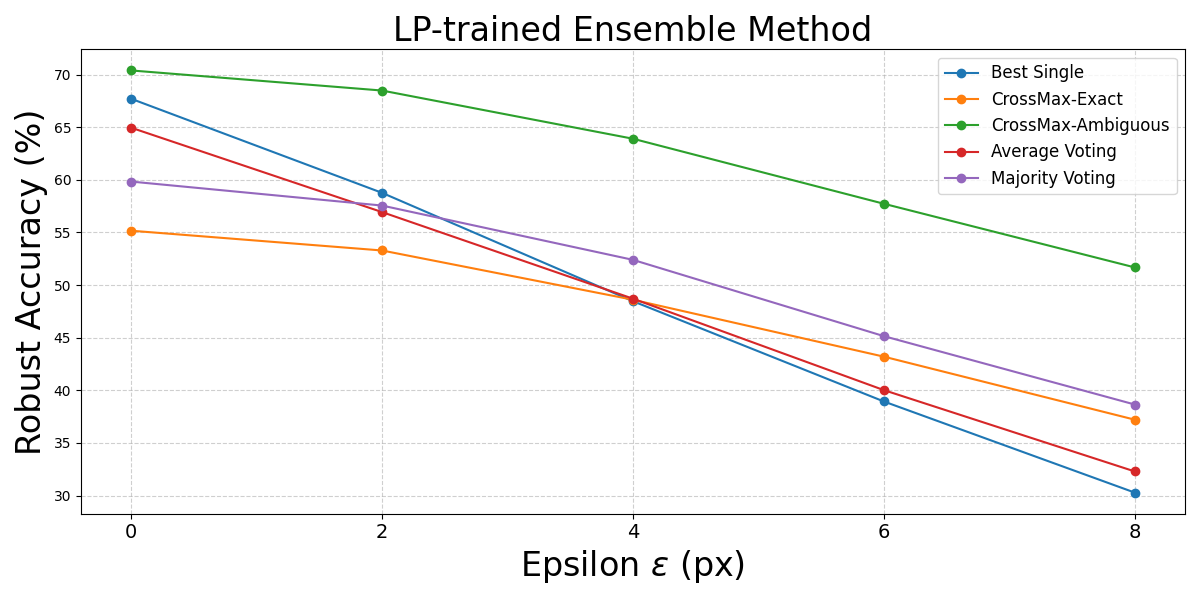
\includegraphics[width=1.0\textwidth]{images/Ensemble LP Performance.png}
    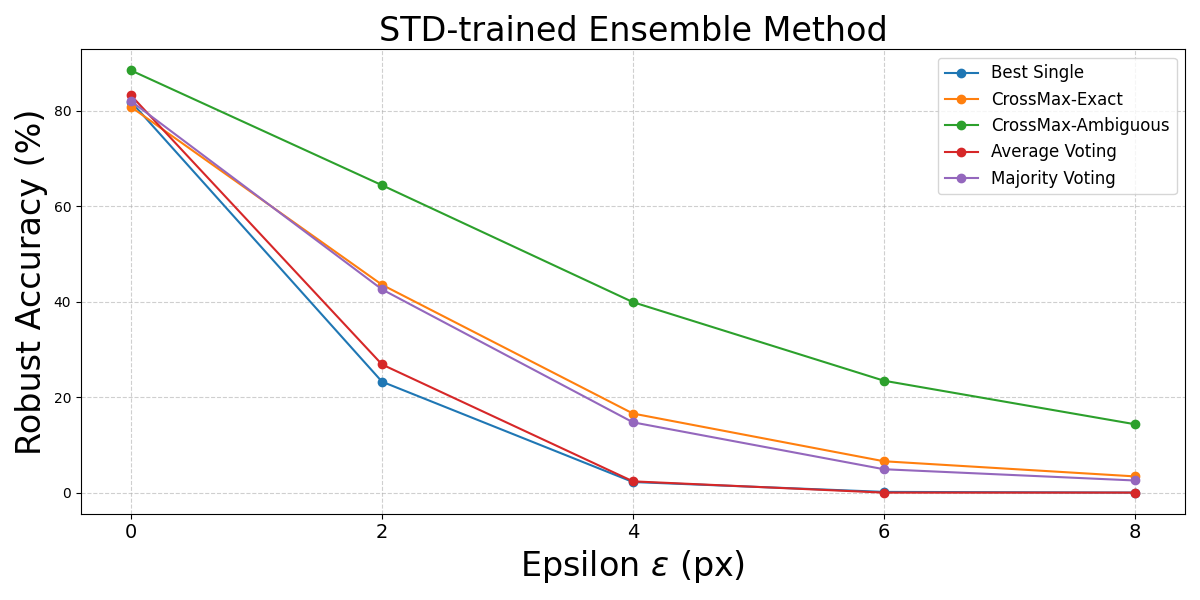
\includegraphics[width=1.0\textwidth]{images/Ensemble STD Performance.png}
    \caption{
    Comparison of ensemble methods vs. the best single model under varying perturbation budgets. 
    Top: ensembles of LP-trained models; Bottom: ensembles of Standard-trained models.
    }

    \label{fig:ensemble_performance}
\end{figure}

\paragraph{Robust Accuracy in Ensemble Methods}
From Tables~\ref{tab:ensemble_lp_compact},  \ref{tab:ensemble_std_compact} and Figure~\ref{fig:ensemble_performance}, we can observe distinct behaviors of the ensemble methods under different perturbation budgets for LP and STD models. For LP models, CrossMax-Ambiguous consistently achieves the highest robust accuracy across all $\epsilon$ values, outperforming the best single model by a notable margin (e.g., +2.69\% at $\epsilon=0$, +21.4\% at $\epsilon=8\mathrm{px}$). The improvement is especially evident at larger perturbation budgets, where the robust accuracy drop is mitigated. The ``Prediction set contains label'' metric remains consistently higher than both the best single model and other ensemble baselines, suggesting that CrossMax-Ambiguous provides more informative prediction sets even when not fully certain. On the other hand, Average Voting and Majority Voting show mixed results: Majority Voting tends to outperform Average Voting at larger $\epsilon$.  
It is worth noting that CrossMax-Exact does not perform as well as expected, particularly under small perturbations where model agreement is relatively high. Compared to CrossMax-Ambiguous, its robust accuracy suffers from the limitation of selecting a single prediction from sets that may contain multiple plausible labels. This shortcoming will be further discussed in Chapter~\ref{chap:conclusion & future work}. Although CrossMax-Ambiguous achieves the best performance in all scenarios, this is obtained under a relaxed prediction requirement. To better understand the characteristics and behavior of its prediction sets, we conducted additional experiments and analyses in the subsequent sections.

For STD models, the advantage of ensemble methods is even more pronounced under adversarial perturbations. CrossMax-Exact offers substantial gains over the best single model starting from $\epsilon=2\mathrm{px}$ (e.g., +20.31\% at $\epsilon=2\mathrm{px}$, +3.39\% at $\epsilon=8\mathrm{px}$). CrossMax-Ambiguous shows the strongest robustness, with large improvements over the best single model across all perturbation budgets, especially in high $\epsilon$ regimes (e.g., +14.32\% absolute robust accuracy at $\epsilon=8\mathrm{px}$). The ``Prediction set contains label'' robust accuracy remains extremely high ($>69\%$) even when the base robust accuracy drops close to zero, indicating its capacity to maintain label coverage under severe perturbations. In contrast, traditional voting methods (Average and Majority) perform significantly worse, particularly for large perturbations, where their robust accuracy approaches that of random guessing.

Overall, CrossMax-Ambiguous emerges as the most effective ensemble method for both LP and STD settings, providing both higher robust accuracy and better label coverage. These results highlight the potential of set-based ensemble predictions in improving robustness under large perturbations, where conventional single-model or simple voting ensembles fail.


\subsection{CrossMax-Ambiguous Prediction Set Size}
\indent

Table~\ref{tab:crossmax_ambiguous} summarizes the average size of the ambiguous prediction sets produced by the CrossMax aggregation method under different perturbation levels for both LP-trained and standard (STD) models. Here, the ambiguous prediction set size refers to the number of classes remaining in the top-$k$ candidates after the CrossMax filtering process, which reflects the model's uncertainty structure from a multi-model perspective.

\begin{table}[h]
\centering
\caption{Average CrossMax-Ambiguous prediction set size under different perturbation budgets.}
\label{tab:crossmax_ambiguous}
\begin{tabular}{c|cc}
\hline
\textbf{Epsilon} & \textbf{LP Model} & \textbf{STD Model} \\
\hline
Clean (0px)   & 1.5768 & 1.2577 \\
2px   & 1.5743 & 1.4665 \\
4px   & 1.5740 & 1.4630 \\
6px   & 1.5737 & 1.3105 \\
8px   & 1.5798 & 1.2117 \\
\hline
\end{tabular}
\end{table}

From Table~\ref{tab:crossmax_ambiguous}, we observe that:
\begin{itemize}
    \item For LP models, the ambiguous set size remains remarkably stable ($\approx 1.57$) across all perturbation levels, indicating that the CrossMax aggregation preserves a consistent level of decision ambiguity even under strong adversarial perturbations.
    \item For STD models, the ambiguous set size is lower than that of LP models when $\epsilon=0$, suggesting higher confidence in clean settings. However, it increases significantly for moderate perturbations ($\epsilon=2,4$) before dropping again at higher perturbations ($\epsilon=6,8$). This pattern suggests that STD models become more uncertain under small-to-moderate attacks, but their predictions collapse to fewer candidate classes under stronger perturbations, potentially due to overconfident misclassification.
\end{itemize}





\subsection{Diversity and Confidence Analysis}  
\label{sec:diversity-confidence-analysis}
\indent

In this section, we analyze and compare the diversity and confidence characteristics of ensembles constructed from two types of base models: LP-trained and standard-trained. We examine how these metrics evolve under varying strengths of adversarial perturbations, providing insights into the robustness mechanisms at play.

Specifically, we first quantify the prediction diversity and ensemble confidence of individual models inside the ensemble as the perturbation budget increases, highlighting differences in their behavior and resilience (Section~\ref{sec:diversity-confidence}). Next, we investigate the CrossMax ensemble method’s ability to produce a unique (single) prediction under different perturbation levels, analyzing how the perturbation strength impacts the CrossMax Confidence score. This offers a nuanced view of prediction ambiguity and certainty in adversarial scenarios.

To contextualize and deepen our understanding, we further compare CrossMax-derived confidence with several traditional ensemble uncertainty and confidence metrics, including softmax-based confidence, prediction entropy, mutual information, and vote agreement. Through this comparative analysis, we aim to reveal correlations and distinctions among these measures and their implications for ensemble robustness.

\begin{table}[htbp]
\centering
\small
\caption{Ensemble Diversity and Confidence Metrics for \textbf{LP-trained} models under varying perturbation budgets.}
\label{tab:diversity_confidence_lp}
\begin{tabular}{lccccc}
\toprule
\textbf{Perturbation} & \textbf{CrossMax Conf.} & \textbf{Diversity} & \textbf{Softmax Conf.} & \textbf{Entropy} & \textbf{Mutual Info.} \\
\midrule
Clean(0px)   & 0.4343 & 0.0057 & 0.3831 & 1.9068 & 0.2259 \\
2px   & 0.4375 & 0.0057 & 0.3823 & 1.9076 & 0.2252 \\
4px   & 0.4400 & 0.0057 & 0.3796 & 1.9107 & 0.2229 \\
6px   & 0.4393 & 0.0057 & 0.3747 & 1.9170 & 0.2188 \\
8px   & 0.4349 & 0.0058 & 0.3689 & 1.9253 & 0.2139 \\
\bottomrule
\end{tabular}
\end{table}


\vspace{1em}

\begin{table}[htbp]
\centering
\small
\caption{Ensemble Diversity and Confidence Metrics for \textbf{STD} models under varying perturbation budgets.}
\label{tab:diversity_confidence_std}
\begin{tabular}{lccccc}
\toprule
\textbf{Perturbation} & \textbf{CrossMax Conf.} & \textbf{Diversity} & \textbf{Softmax Conf.} & \textbf{Entropy} & \textbf{Mutual Info.} \\
\midrule
Clean(0px)   & 0.7517 & 0.0026 & 0.7704 & 0.8133 & 0.1733 \\
2px   & 0.5484 & 0.0038 & 0.7551 & 0.9116 & 0.2459 \\
4px   & 0.5455 & 0.0038 & 0.7771 & 0.8978 & 0.2947 \\
6px   & 0.6957 & 0.0028 & 0.8161 & 0.7547 & 0.2506 \\
8px   & 0.7940 & 0.0021 & 0.8448 & 0.6328 & 0.2019 \\
\bottomrule
\end{tabular}
\end{table}






\paragraph{Diversity and Confidence in LP vs. Standard Ensembles}

Tables~\ref{tab:diversity_confidence_std} and~\ref{tab:diversity_confidence_lp} summarize key ensemble metrics for standard-trained (STD) and LP-trained models under varying perturbation budgets. 

We observe that the LP-trained ensembles consistently exhibit higher prediction diversity than the STD-trained ones across all perturbation levels, with diversity values around 0.0057–0.0058 compared to the STD’s lower range of 0.0021–0.0038. This indicates that LP training encourages more heterogeneous network predictions inside ensemble model, which can contribute to robustness against adversarial transferability.

In contrast, confidence metrics such as CrossMax Confidence and Softmax Confidence are notably higher for the STD ensembles, especially at larger perturbations (e.g., at 8px, CrossMax Confidence reaches 0.7940 for STD vs. 0.4349 for LP). Correspondingly, the STD models tend to have lower prediction entropy, suggesting more confident and sharper ensemble predictions compared to LP models, which maintain high entropy values (~about 1.9), indicative of greater uncertainty.

MI, reflecting epistemic uncertainty and model disagreement, exhibits smaller variation in LP-trained ensembles compared to standard ensembles, suggesting more consistent behavior among networks inside ensemble models despite their robustness-oriented training. Similarly, entropy values for LP-trained ensembles remain consistently high (around 1.90–1.92) across perturbation budgets, indicating uniformly distributed predictions and limited confidence shifts. In contrast, entropy in standard ensembles fluctuates sharply (from 0.81 at clean inputs to 0.91 and then dropping to 0.63), highlighting greater volatility in predictive confidence under adversarial perturbations.

However, as observed from Tables~\ref{tab:ensemble_lp_compact} and \ref{tab:ensemble_std_compact}, high confidence does not necessarily imply reliable predictions. This “confidence” can be substantially misleading when all models are extensively fooled by strong attacks. For instance, under the 8px attack on the STD ensemble, despite the model exhibiting high self-confidence in its predictions (CrossMax Confidence of 0.7940), the actual ensemble performance deteriorates drastically, with majority voting accuracy plummeting to only 2.55\%. This highlights the gap between confidence measures and true robustness under adversarial conditions.


\paragraph{CrossMax Confidence and Softmax Confidence under Perturbations}

To further explore ensemble confidence dynamics, we compare CrossMax Confidence with Softmax Confidence as perturbation strength varies, using the two figures shown in Figures~\ref{fig:softmax_confidence} and ~\ref{fig:crossmax_confidence}. Both plots illustrate the trend of confidence scores for LP-trained and standard-trained ensembles under increasing adversarial budgets.

We observe that the more robust LP-trained ensembles maintain remarkably stable confidence scores across both metrics, with fluctuations on the order of $10^{-2}$. In contrast, the STD-trained ensembles, which are more susceptible to adversarial perturbations, show notably larger variability in confidence. For both CrossMax and Softmax Confidence, the STD models exhibit a non-monotonic trend: confidence first decreases as attacks grow stronger, then increases again when perturbations become large enough to deceive most networks inside the ensemble model simultaneously.

Interestingly, this characteristic pattern is more pronounced in CrossMax Confidence than in Softmax Confidence. According to Table~\ref{tab:diversity_confidence_std}, the absolute change in Softmax Confidence across perturbations is approximately 0.0897, whereas CrossMax Confidence demonstrates a larger absolute difference of 0.2485. This suggests that CrossMax Confidence captures the ensemble’s shifting certainty more sensitively under adversarial conditions, potentially providing a more informative measure of robustness compared to traditional softmax-based confidence.



\begin{figure}[H]
    \centering
    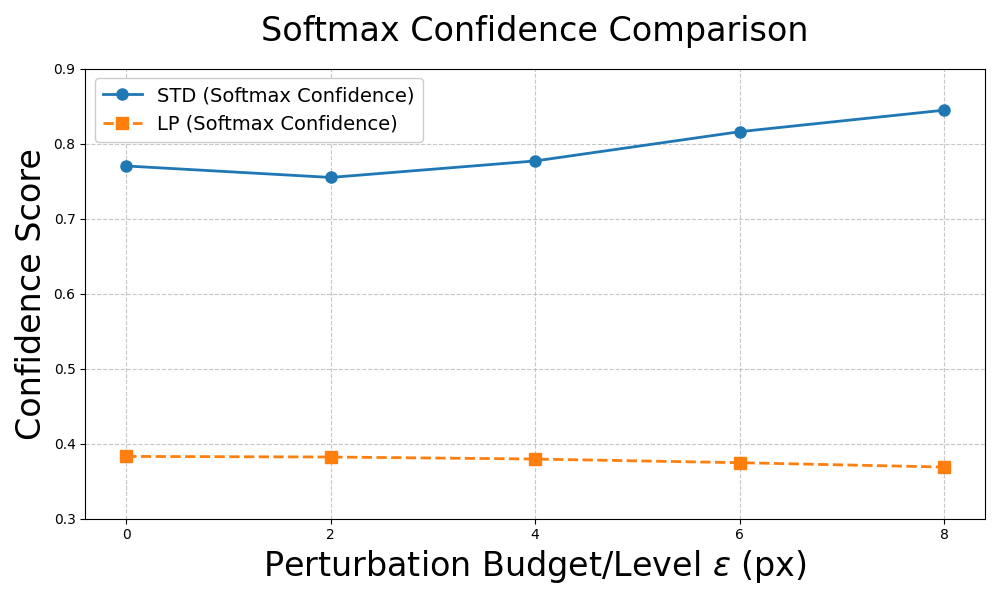
\includegraphics[width=0.8\linewidth]{images/SoftMax Confidence.png}
    \caption{Softmax Confidence scores for LP-trained and STD-trained ensembles as perturbation budget increases.}
    \label{fig:softmax_confidence}
\end{figure}

\begin{figure}[H]
    \centering
    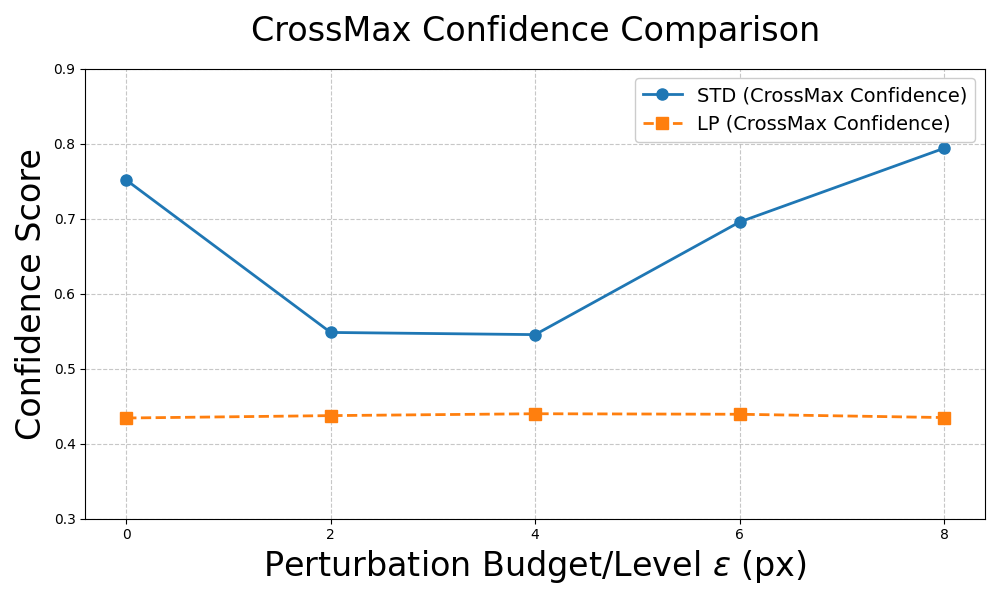
\includegraphics[width=0.8\linewidth]{images/CrossMax Confidence.png}
    \caption{CrossMax Confidence scores for LP-trained and STD-trained ensembles as perturbation budget increases.}
    \label{fig:crossmax_confidence}
\end{figure}


\section{Discussion}
\label{sec:discussion}
\indent

This section synthesizes the experimental findings and interprets their implications for ensemble robustness under adversarial perturbations, with a particular focus on differences between LP-trained and standard-trained models, the impact of model architectures, and the effectiveness of various ensemble strategies and confidence metrics.

\paragraph{Robustness and Accuracy Trade-offs in LP Training}

Consistent with prior literature~\cite{li2023sok}, LP-trained models exhibit a well-known trade-off between clean accuracy and certified robustness. Our results demonstrate that LP training improves adversarial robustness substantially compared to standard training, especially at higher perturbation budgets. However, this robustness gain comes at the cost of reduced clean accuracy, highlighting a fundamental tension in adversarial defenses. Moreover, the perturbation budget used during training critically shapes the robustness profile: models trained with smaller budgets perform better under light perturbations but degrade quickly as attacks intensify, while models trained with larger budgets show more stable performance across all perturbations despite lower clean accuracy.

\paragraph{Model Architecture Effects on Robustness}

Our analysis reveals that the impact of model architecture on robustness is nuanced and depends heavily on the training regime. For LP-trained models, ResNet architectures generally achieve a better balance of robustness and stability across perturbations, while Large models underperform at higher budgets possibly due to over-regularization or optimization challenges. Conversely, in the absence of robust training, smaller models appear more stable against increasing perturbations, though their absolute robust accuracy remains low. This suggests that architectural complexity interacts with training strategy to influence robustness characteristics in non-trivial ways.

\paragraph{Ensemble Methods and Their Robustness Benefits}

Across both LP and standard training, set-based ensemble methods CrossMax-Ambiguous, outperform traditional averaging or majority voting approaches in robust accuracy, especially at higher perturbation levels. This indicates that relaxing the ensemble prediction to a set of plausible labels can effectively mitigate the sharp accuracy drop-off caused by strong adversarial attacks. Notably, CrossMax-Exact underperforms when perturbations are small and networks agreement inside the ensemble model is high, likely due to its restrictive single-label output. The advantage of CrossMax-Ambiguous highlights the potential of incorporating prediction ambiguity into ensemble robustness strategies.

\paragraph{Ambiguity in CrossMax Ensemble Predictions}

The ambiguous prediction set size produced by CrossMax aggregation reveals contrasting behaviors between LP and standard ensembles. LP-trained ensembles maintain a stable ambiguous set size (~around 1.57 classes), even as perturbations increase, suggesting preserved decision diversity and calibrated uncertainty. In contrast, standard-trained ensembles exhibit a non-monotonic trend in ambiguity: initial high confidence on clean data gives way to increased ambiguity at moderate perturbations, followed by a collapse to fewer candidate classes under strong attacks. This pattern reflects a breakdown in confidence calibration and growing overconfidence in erroneous predictions as attacks intensify.

\paragraph{Diversity and Confidence Metrics under Perturbations}

LP-trained ensembles consistently exhibit higher prediction diversity than standard-trained ones, reflecting more heterogeneous network outputs inside the ensemble model which may aid robustness against transferable adversarial perturbations. Standard-trained ensembles show higher CrossMax and Softmax confidence, especially at large perturbations, but this confidence is often misleading. For example, under strong attacks, the standard ensemble's CrossMax Confidence remains high while actual accuracy plummets, evidencing overconfident yet unreliable predictions.

Further analysis of confidence dynamics shows that LP-trained ensembles maintain remarkably stable confidence across perturbation strengths, with minimal fluctuations in both CrossMax and Softmax metrics. In contrast, standard-trained ensembles experience pronounced confidence oscillations: confidence dips as perturbations grow stronger, then rises again when most networks inside the ensemble model are fooled. This non-monotonic behavior is more evident in CrossMax Confidence than Softmax Confidence, suggesting that CrossMax metrics may better capture the ensemble’s shifting uncertainty and provide a more sensitive indicator of robustness under adversarial conditions.

\paragraph{Summary}

Overall, our study underscores the complex interplay between training strategies, model architecture, ensemble methods, and confidence measures in shaping adversarial robustness. LP training and sophisticated ensemble approaches like CrossMax-Ambiguous improve robustness but highlight the need for careful confidence calibration and ambiguity-aware predictions. The observed limitations of standard confidence metrics and traditional ensemble voting suggest promising directions for future research, including the development of more reliable confidence indicators and adaptive ensemble aggregation techniques tailored for adversarial resilience.